% Options for packages loaded elsewhere
\PassOptionsToPackage{unicode}{hyperref}
\PassOptionsToPackage{hyphens}{url}
%
\documentclass[
]{book}
\usepackage{amsmath,amssymb}
\usepackage{lmodern}
\usepackage{iftex}
\ifPDFTeX
  \usepackage[T1]{fontenc}
  \usepackage[utf8]{inputenc}
  \usepackage{textcomp} % provide euro and other symbols
\else % if luatex or xetex
  \usepackage{unicode-math}
  \defaultfontfeatures{Scale=MatchLowercase}
  \defaultfontfeatures[\rmfamily]{Ligatures=TeX,Scale=1}
\fi
% Use upquote if available, for straight quotes in verbatim environments
\IfFileExists{upquote.sty}{\usepackage{upquote}}{}
\IfFileExists{microtype.sty}{% use microtype if available
  \usepackage[]{microtype}
  \UseMicrotypeSet[protrusion]{basicmath} % disable protrusion for tt fonts
}{}
\makeatletter
\@ifundefined{KOMAClassName}{% if non-KOMA class
  \IfFileExists{parskip.sty}{%
    \usepackage{parskip}
  }{% else
    \setlength{\parindent}{0pt}
    \setlength{\parskip}{6pt plus 2pt minus 1pt}}
}{% if KOMA class
  \KOMAoptions{parskip=half}}
\makeatother
\usepackage{xcolor}
\usepackage{color}
\usepackage{fancyvrb}
\newcommand{\VerbBar}{|}
\newcommand{\VERB}{\Verb[commandchars=\\\{\}]}
\DefineVerbatimEnvironment{Highlighting}{Verbatim}{commandchars=\\\{\}}
% Add ',fontsize=\small' for more characters per line
\usepackage{framed}
\definecolor{shadecolor}{RGB}{248,248,248}
\newenvironment{Shaded}{\begin{snugshade}}{\end{snugshade}}
\newcommand{\AlertTok}[1]{\textcolor[rgb]{0.94,0.16,0.16}{#1}}
\newcommand{\AnnotationTok}[1]{\textcolor[rgb]{0.56,0.35,0.01}{\textbf{\textit{#1}}}}
\newcommand{\AttributeTok}[1]{\textcolor[rgb]{0.77,0.63,0.00}{#1}}
\newcommand{\BaseNTok}[1]{\textcolor[rgb]{0.00,0.00,0.81}{#1}}
\newcommand{\BuiltInTok}[1]{#1}
\newcommand{\CharTok}[1]{\textcolor[rgb]{0.31,0.60,0.02}{#1}}
\newcommand{\CommentTok}[1]{\textcolor[rgb]{0.56,0.35,0.01}{\textit{#1}}}
\newcommand{\CommentVarTok}[1]{\textcolor[rgb]{0.56,0.35,0.01}{\textbf{\textit{#1}}}}
\newcommand{\ConstantTok}[1]{\textcolor[rgb]{0.00,0.00,0.00}{#1}}
\newcommand{\ControlFlowTok}[1]{\textcolor[rgb]{0.13,0.29,0.53}{\textbf{#1}}}
\newcommand{\DataTypeTok}[1]{\textcolor[rgb]{0.13,0.29,0.53}{#1}}
\newcommand{\DecValTok}[1]{\textcolor[rgb]{0.00,0.00,0.81}{#1}}
\newcommand{\DocumentationTok}[1]{\textcolor[rgb]{0.56,0.35,0.01}{\textbf{\textit{#1}}}}
\newcommand{\ErrorTok}[1]{\textcolor[rgb]{0.64,0.00,0.00}{\textbf{#1}}}
\newcommand{\ExtensionTok}[1]{#1}
\newcommand{\FloatTok}[1]{\textcolor[rgb]{0.00,0.00,0.81}{#1}}
\newcommand{\FunctionTok}[1]{\textcolor[rgb]{0.00,0.00,0.00}{#1}}
\newcommand{\ImportTok}[1]{#1}
\newcommand{\InformationTok}[1]{\textcolor[rgb]{0.56,0.35,0.01}{\textbf{\textit{#1}}}}
\newcommand{\KeywordTok}[1]{\textcolor[rgb]{0.13,0.29,0.53}{\textbf{#1}}}
\newcommand{\NormalTok}[1]{#1}
\newcommand{\OperatorTok}[1]{\textcolor[rgb]{0.81,0.36,0.00}{\textbf{#1}}}
\newcommand{\OtherTok}[1]{\textcolor[rgb]{0.56,0.35,0.01}{#1}}
\newcommand{\PreprocessorTok}[1]{\textcolor[rgb]{0.56,0.35,0.01}{\textit{#1}}}
\newcommand{\RegionMarkerTok}[1]{#1}
\newcommand{\SpecialCharTok}[1]{\textcolor[rgb]{0.00,0.00,0.00}{#1}}
\newcommand{\SpecialStringTok}[1]{\textcolor[rgb]{0.31,0.60,0.02}{#1}}
\newcommand{\StringTok}[1]{\textcolor[rgb]{0.31,0.60,0.02}{#1}}
\newcommand{\VariableTok}[1]{\textcolor[rgb]{0.00,0.00,0.00}{#1}}
\newcommand{\VerbatimStringTok}[1]{\textcolor[rgb]{0.31,0.60,0.02}{#1}}
\newcommand{\WarningTok}[1]{\textcolor[rgb]{0.56,0.35,0.01}{\textbf{\textit{#1}}}}
\usepackage{longtable,booktabs,array}
\usepackage{calc} % for calculating minipage widths
% Correct order of tables after \paragraph or \subparagraph
\usepackage{etoolbox}
\makeatletter
\patchcmd\longtable{\par}{\if@noskipsec\mbox{}\fi\par}{}{}
\makeatother
% Allow footnotes in longtable head/foot
\IfFileExists{footnotehyper.sty}{\usepackage{footnotehyper}}{\usepackage{footnote}}
\makesavenoteenv{longtable}
\usepackage{graphicx}
\makeatletter
\def\maxwidth{\ifdim\Gin@nat@width>\linewidth\linewidth\else\Gin@nat@width\fi}
\def\maxheight{\ifdim\Gin@nat@height>\textheight\textheight\else\Gin@nat@height\fi}
\makeatother
% Scale images if necessary, so that they will not overflow the page
% margins by default, and it is still possible to overwrite the defaults
% using explicit options in \includegraphics[width, height, ...]{}
\setkeys{Gin}{width=\maxwidth,height=\maxheight,keepaspectratio}
% Set default figure placement to htbp
\makeatletter
\def\fps@figure{htbp}
\makeatother
\setlength{\emergencystretch}{3em} % prevent overfull lines
\providecommand{\tightlist}{%
  \setlength{\itemsep}{0pt}\setlength{\parskip}{0pt}}
\setcounter{secnumdepth}{5}
\usepackage{booktabs}
\usepackage{amsthm}
\makeatletter
\def\thm@space@setup{%
  \thm@preskip=8pt plus 2pt minus 4pt
  \thm@postskip=\thm@preskip
}
\makeatother
\ifLuaTeX
  \usepackage{selnolig}  % disable illegal ligatures
\fi
\usepackage[]{natbib}
\bibliographystyle{apalike}
\IfFileExists{bookmark.sty}{\usepackage{bookmark}}{\usepackage{hyperref}}
\IfFileExists{xurl.sty}{\usepackage{xurl}}{} % add URL line breaks if available
\urlstyle{same} % disable monospaced font for URLs
\hypersetup{
  pdftitle={Business Analyst in Teams},
  pdfauthor={Team 3: We Also Hate Python},
  hidelinks,
  pdfcreator={LaTeX via pandoc}}

\title{Business Analyst in Teams}
\author{Team 3: We Also Hate Python}
\date{2022-07-18}

\begin{document}
\maketitle

{
\setcounter{tocdepth}{1}
\tableofcontents
}
\hypertarget{preface}{%
\chapter{Preface}\label{preface}}

Business Analyst in Teams

\begin{Shaded}
\begin{Highlighting}[]
\CommentTok{\# maybe add a pic here as a cover for the book}
\end{Highlighting}
\end{Shaded}

\hypertarget{introduction}{%
\chapter{Introduction}\label{introduction}}

\hypertarget{introduction-and-background}{%
\section{\texorpdfstring{\textbf{Introduction and Background}}{Introduction and Background}}\label{introduction-and-background}}

Too often, we find ourselves learning how to recruit and network to land jobs when in reality we do not know the full responsibilities a role entails. Since we are the first cohort of the MBAn program, all our peers and future MBAn students most likely consider some variation of business analytics role as their immediate career option. Our project aims to develop a broad framework to understand and navigate the Business Analyst role in different industries such as Consulting, Finance, and Tech, with an emphasis on how Business Analyst works in team settings.

~

\hypertarget{purpose-and-objective}{%
\section{\texorpdfstring{\textbf{Purpose and Objective}}{Purpose and Objective}}\label{purpose-and-objective}}

The purpose of this project is to gain valuable insights into the specific responsibilities of a business analyst in different industries, which we can use in the coming months to choose a career path. The objective is to understand the responsibilities and skills needed to work in these fields including both technical and soft skills. From there, the objective is to understand the nature of the team. We are interested in the growth and future of different positions, and finally, work/life balance.

~

\hypertarget{plan}{%
\section{\texorpdfstring{\textbf{Plan}}{Plan}}\label{plan}}

\begin{itemize}
\tightlist
\item
  Conduct independent research on the roles and responsibilities of analysts and how they interact with other professionals in the same team.
\item
  Network and interview 3 different analysts in different industries.
\end{itemize}

\hypertarget{project-deliverables}{%
\section{\texorpdfstring{\textbf{Project Deliverables}}{Project Deliverables}}\label{project-deliverables}}

\begin{itemize}
\tightlist
\item
  A RMarkdown document about 20 pages long
\item
  A presentation slides
\end{itemize}

\hypertarget{interview-leads}{%
\section{\texorpdfstring{\textbf{Interview Leads}}{Interview Leads}}\label{interview-leads}}

\begin{quote}
\hypertarget{consulting}{%
\subsection{\texorpdfstring{\textbf{Consulting}}{Consulting}}\label{consulting}}

\begin{itemize}
\tightlist
\item
  McKinsey
\item
  ZS Solutions
\item
  EY (tech consulting)
\end{itemize}
\end{quote}

\begin{quote}
\hypertarget{finance}{%
\subsection{\texorpdfstring{\textbf{Finance}}{Finance}}\label{finance}}

\begin{itemize}
\tightlist
\item
  Jackson National
\item
  JP Morgan
\item
  Goldman Sachs
\end{itemize}
\end{quote}

\begin{quote}
\hypertarget{tech}{%
\subsection{\texorpdfstring{\textbf{Tech}}{Tech}}\label{tech}}

\begin{itemize}
\tightlist
\item
  Google
\item
  Amazon
\item
  Microsoft
\end{itemize}
\end{quote}

\hypertarget{timeline}{%
\section{\texorpdfstring{\textbf{Timeline}}{Timeline}}\label{timeline}}

\begin{itemize}
\tightlist
\item
  Proposal: July 20th
\item
  Interviews due: Aug 10th
\item
  Group Project Specification: Aug 15th
\item
  Group Project Presentation (ppt submission): Aug 16th
\end{itemize}

\hypertarget{about-us}{%
\chapter{About Us}\label{about-us}}

\hypertarget{team-3-we-also-hate-python-aka-mjjjj}{%
\section{Team 3: We Also Hate Python (aka MJJJJ)}\label{team-3-we-also-hate-python-aka-mjjjj}}

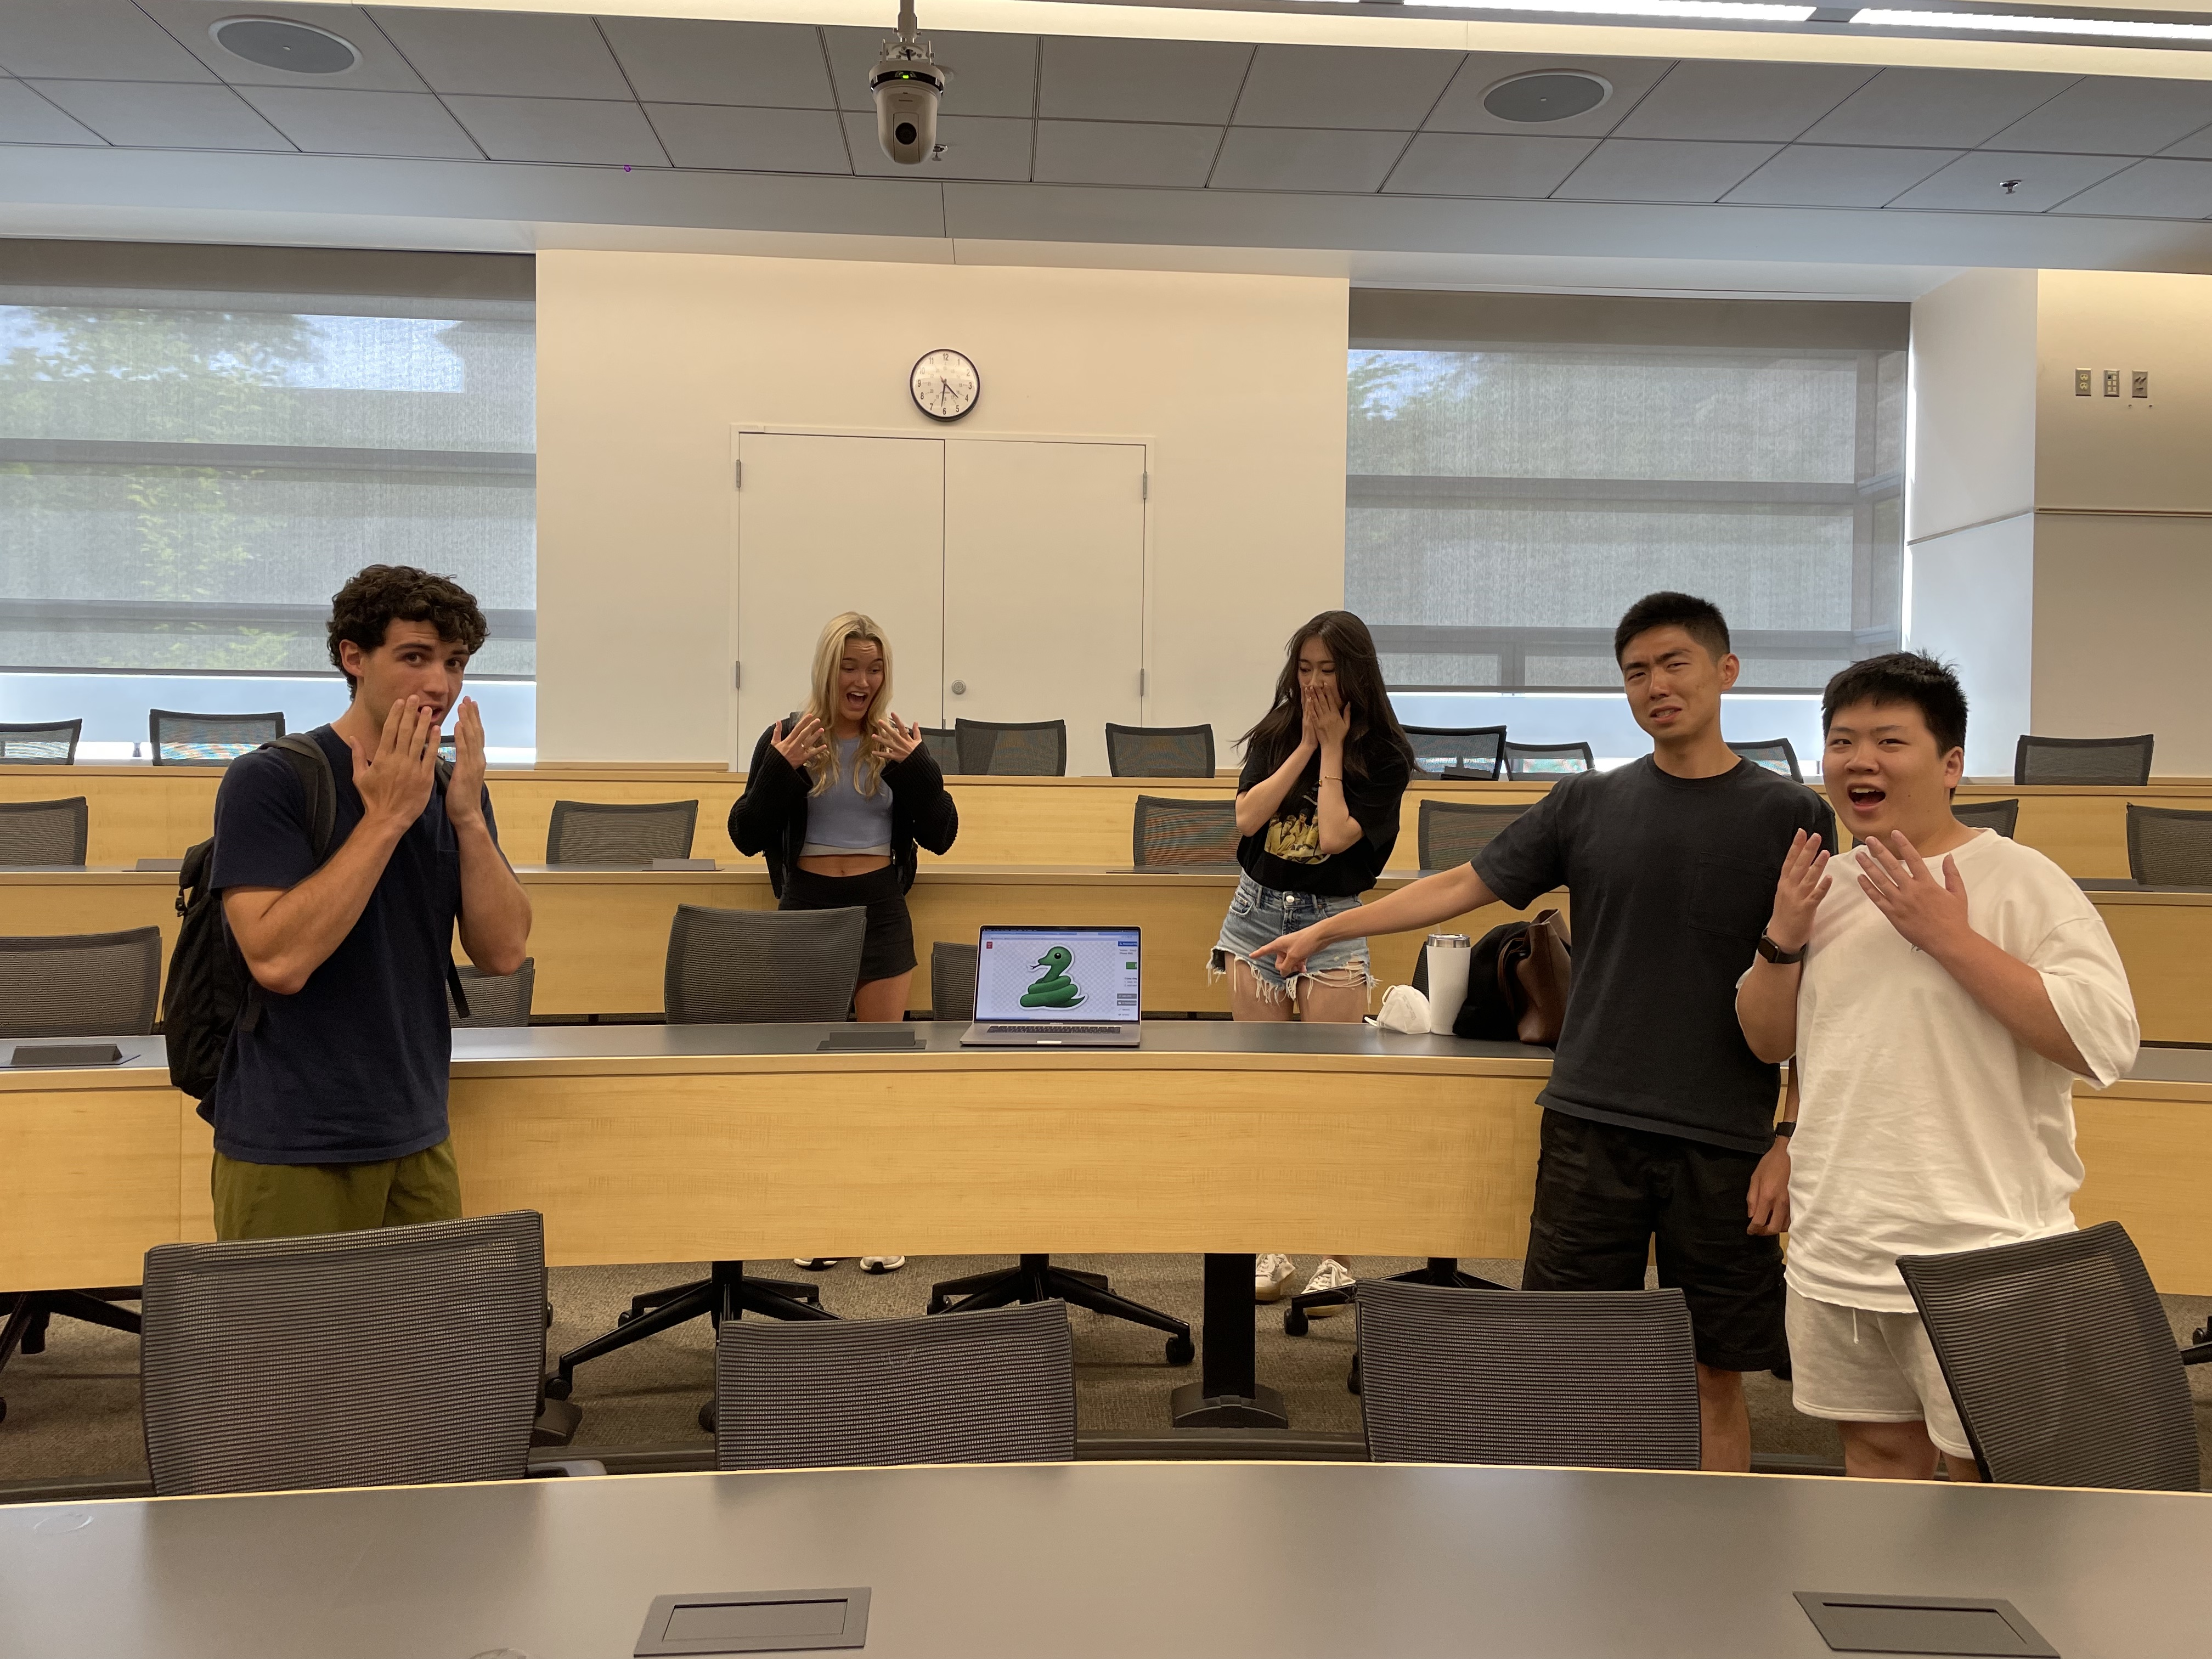
\includegraphics[width=1\linewidth]{_pictures/about_us/team_pic}

\hypertarget{madison-hartle}{%
\section{Madison Hartle}\label{madison-hartle}}

I am a recent graduate from the University of Michigan where I earned a bachelor's degree in Actuarial Mathematics. Currently, I am pursuing a masters degree in Business Analytics.

\hypertarget{general-information}{%
\subsection{General Information}\label{general-information}}

Here is a list of things that I enjoy:

\begin{itemize}
\tightlist
\item
  Long walks in the Arb
\item
  Traveling
\item
  Spending time with friends and family
\item
  Reading novels
\item
  Writing poetry
\item
  Eating ice cream
\end{itemize}

\hypertarget{some-things-you-probably-didnt-know}{%
\subsection{Some things you probably didn't know}\label{some-things-you-probably-didnt-know}}

\begin{enumerate}
\def\labelenumi{\arabic{enumi}.}
\tightlist
\item
  My birthday is February 7th, 2000
\item
  I've been bungee jumping twice
\item
  I'm a math major but I didn't learn how to long divide until I was in college
\item
  The Mackinac Bridge is 500 feet high and 5 miles long
\end{enumerate}

\begin{figure}
\includegraphics[width=0.5\linewidth]{_pictures/about_us/Mattie} \caption{A break from skiing.}\label{fig:pic-Mattie}
\end{figure}

\hypertarget{jenny-yajie-xu}{%
\section{Jenny (Yajie) Xu}\label{jenny-yajie-xu}}

\hypertarget{basic-information}{%
\subsection{Basic Information}\label{basic-information}}

\textbf{First Name}: Yajie

\textbf{Last Name}: Xu

\textbf{Preferred Name}: Jenny

\textbf{Age}: 22

\textbf{Birthday}: 04/03/2000

\textbf{School}: Ross School of Business

\textbf{Field of Study}: MBAn

\textbf{Favorite Coding Language}: R

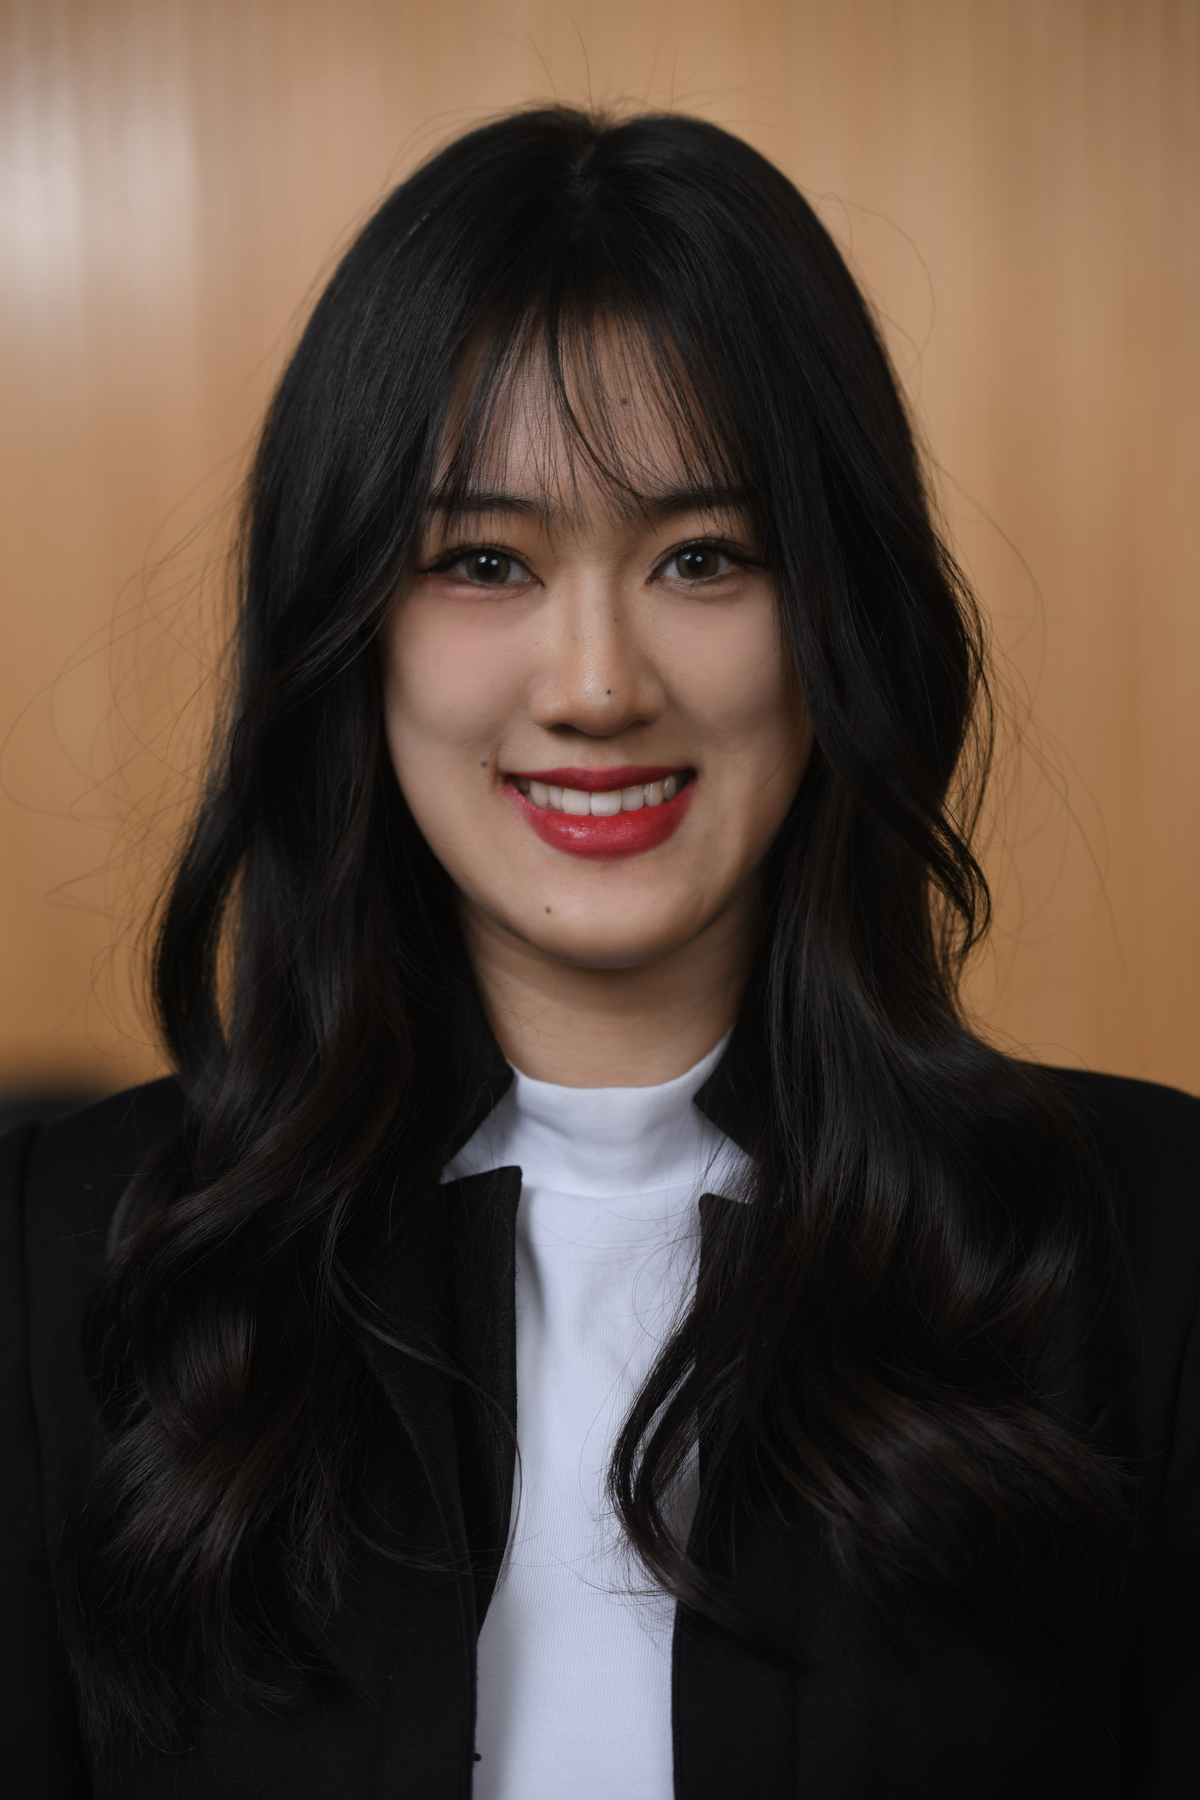
\includegraphics[width=0.3\linewidth]{_pictures/about_us/Jenny}

\hypertarget{john-oraa}{%
\section{John Oraa}\label{john-oraa}}

\begin{figure}
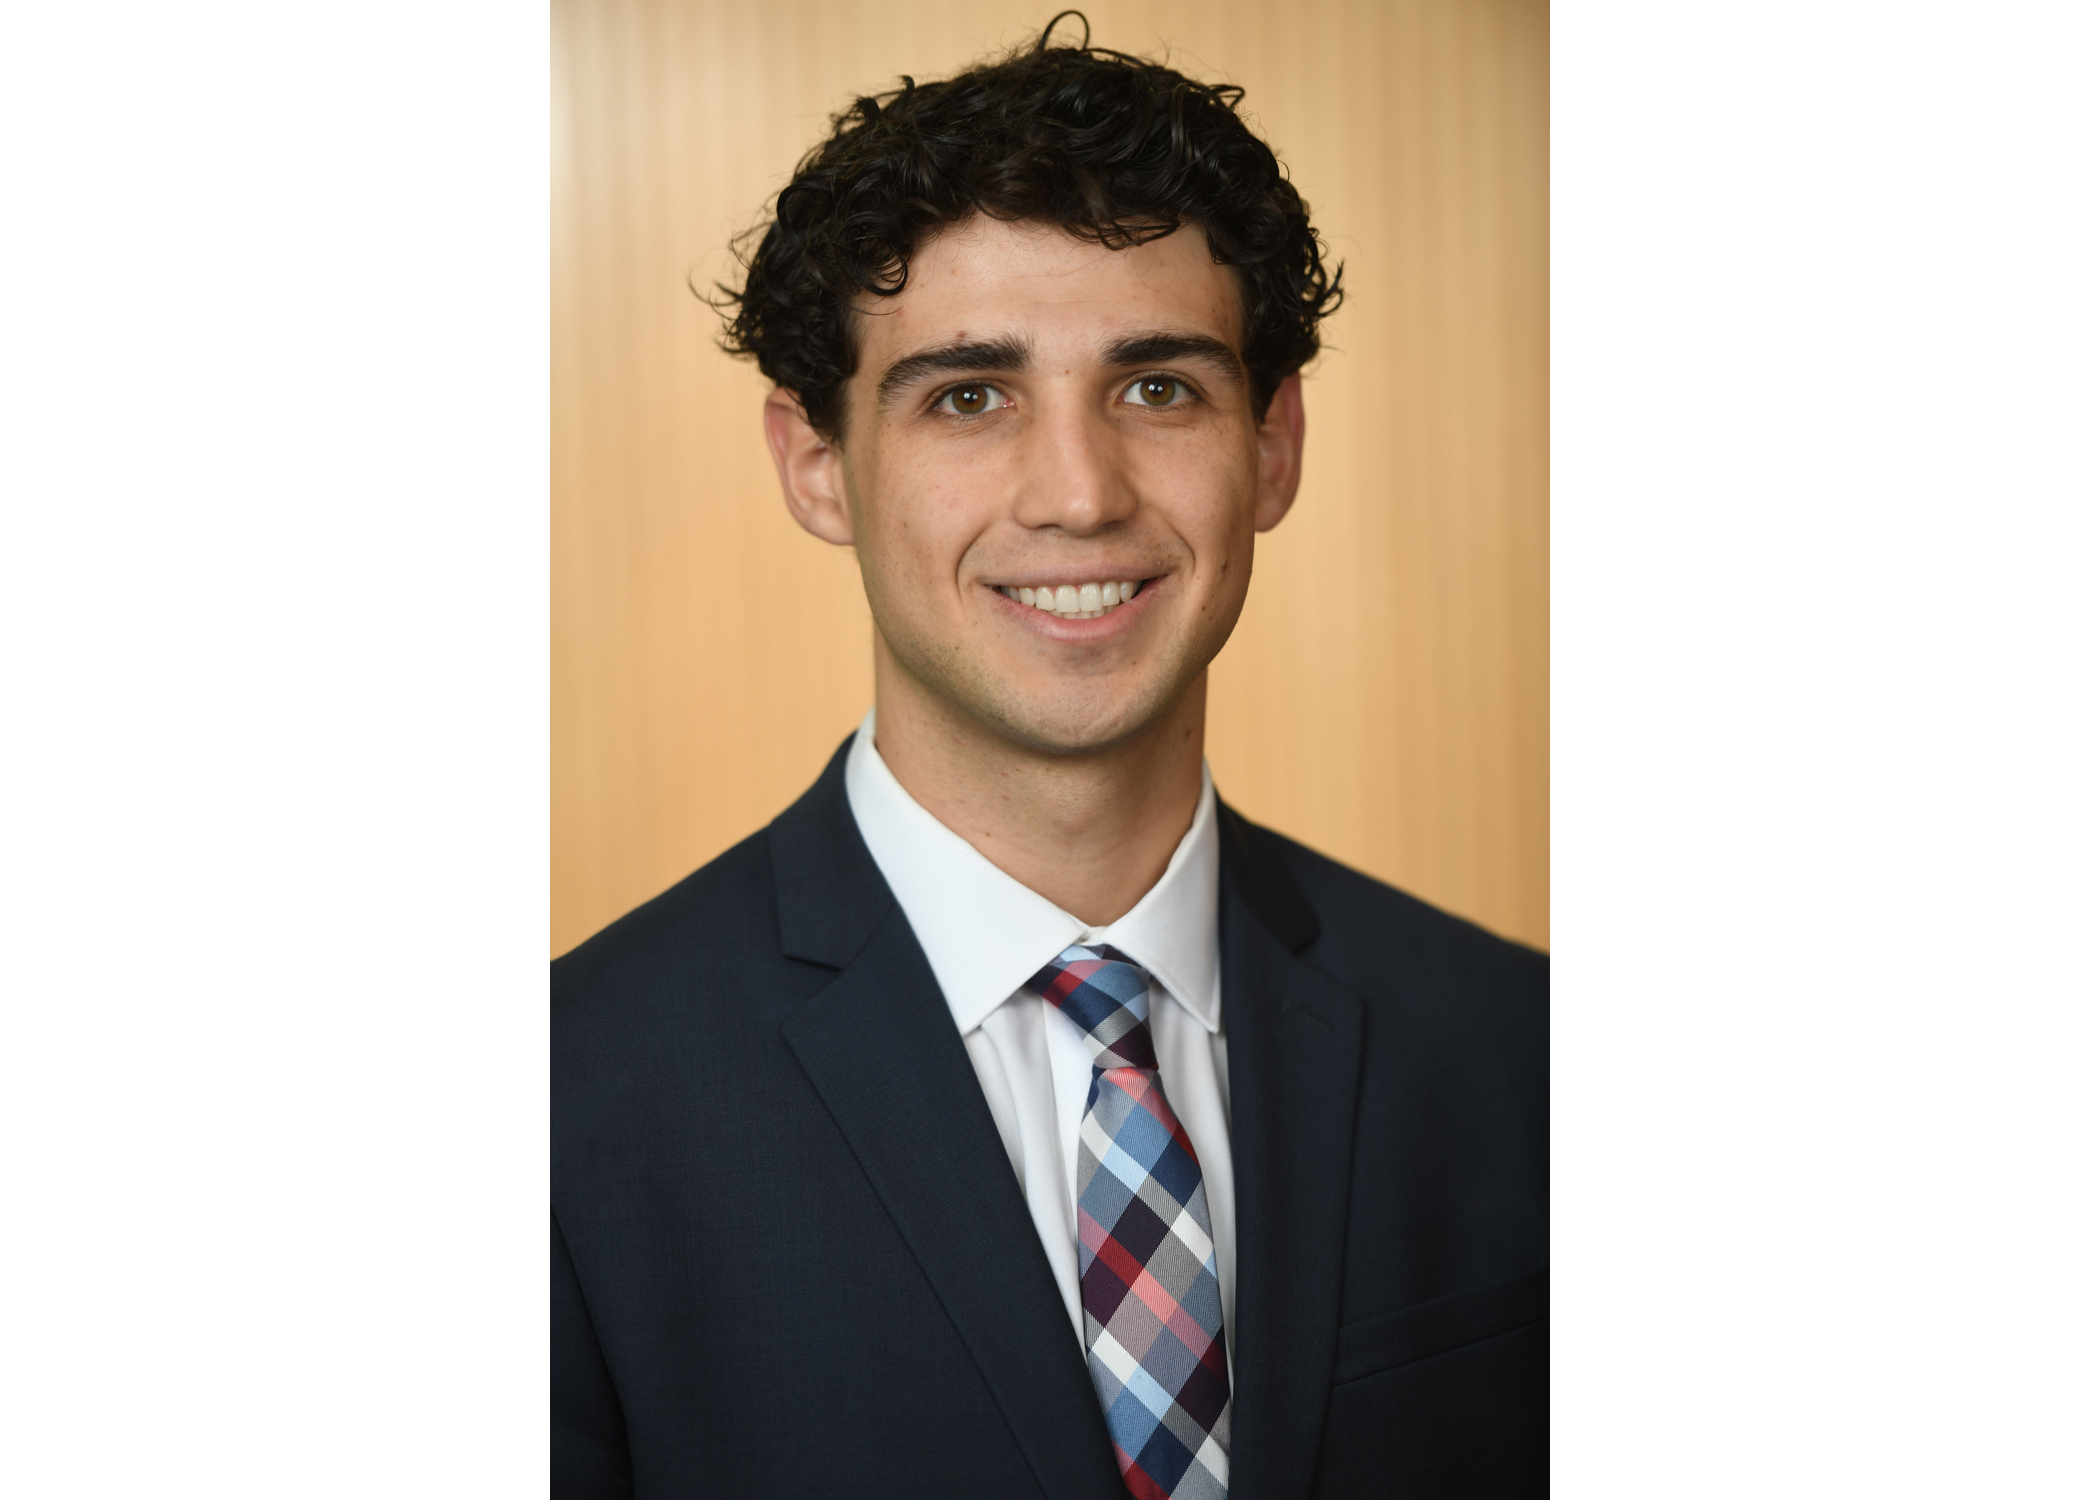
\includegraphics[width=0.8\linewidth]{_pictures/about_us/John} \caption{John Oraa MBAn Class of 2023.}\label{fig:pic-John}
\end{figure}

\hypertarget{my-life}{%
\subsection{My Life}\label{my-life}}

Hello! My name is John. I am a 22 year old from a small town in Michigan called Fenton. Recently, I just graduated from the University of Michigan with my B.S.E in Mechanical Engineering. I recently began my masters at the Ross School of Business studying Business Analytics.

My goal is to combine my technical undergraduate skills and master degree to focus my efforts on improving the business of healthcare.

\hypertarget{my-accomlishments}{%
\subsection{My Accomlishments}\label{my-accomlishments}}

\hypertarget{project-teams}{%
\subsubsection{Project Teams}\label{project-teams}}

In my undergrad I was apart of a couple different design teams focusing on engineering and consulting our customer

\begin{itemize}
\tightlist
\item
  Medlaunch which focused on developing a need based issue in our community through consulting with our community partner
\item
  STARX which is the exoskeleton project engineering team developing an exoskeleton to be used in assisting Parkinsons patients
\end{itemize}

\hypertarget{professional-experience}{%
\subsubsection{Professional Experience}\label{professional-experience}}

\begin{itemize}
\item
  Research: I have conducted research in human walking gait identification, parkinson's patients foot fall detection, mesh morphing.
\item
  Engineering Design Internship
\item
  Commercial Sale/Business Analytics Experience
\end{itemize}

\hypertarget{jason-xiaodi-pan}{%
\section{Jason (Xiaodi) Pan}\label{jason-xiaodi-pan}}

\hypertarget{background}{%
\subsection{Background}\label{background}}

Hey everyone, my name is Xiaodi Pan and people usually call me Jason.

I was born and raised in Shanghai, China and I came to the U.S in 2016 for high school. I graduated from Penn State University in Spring 2022 with a major in Supply Chain Management and a minor in Information System Management. I am currently a Master's of Business Analytic student at University of Michigan Ross School of Business.

\href{https://www.linkedin.com/in/xiaodi-jason-pan/}{Learn more about me professionally through Linkedin!}

I am actively looking for job opportunities in consulting, finance, supply chain and all other related areas in business. I'd love to own a consulting firm that focuses on innovative supply chain solutions for companies in the industry one day.

\begin{figure}
\includegraphics[width=0.5\linewidth]{_pictures/about_us/Jason} \caption{Just me and my friend reflecting on life and Yes I was the one wearing shorts}\label{fig:pic-Jason}
\end{figure}

\hypertarget{fun-facts}{%
\subsection{Fun Facts!!!}\label{fun-facts}}

\begin{itemize}
\tightlist
\item
  I speak fluent Shanghainese and learned Spanish for 3 years
\item
  I am a basketball and soccer fan and my favorite teams are Golden State Warriors and Manchester United
\item
  I spend a lot of my spare time watching movies and TV shows. My favourite TV show of all time is \emph{Prison Break}
\item
  I love racing. I drive a 6 Speed 2021 Booster Blue Honda Civic Type R and I also like to sim-race when I'm free
\item
  Formula 1 is one of my favorite sports and I root for Daniel Riccardo and Charles Leclerc
\item
  I co-own a company called \emph{Lorna Kicks} and we source fashion sneakers, street wears and electronics for clients
\end{itemize}

\begin{figure}
\includegraphics[width=0.5\linewidth]{_pictures/about_us/Jason_car} \caption{My baby :) }\label{fig:pic-Jason-car}
\end{figure}

\hypertarget{referral-links-not-financial-advice}{%
\subsection{\texorpdfstring{Referral Links (\textbf{Not Financial Advice})}{Referral Links (Not Financial Advice)}}\label{referral-links-not-financial-advice}}

\begin{quote}
\href{https://www.youtube.com/watch?v=dQw4w9WgXcQ}{How I obtained 850+ credit score at the age of 14 (I don't share this with many people)}
\end{quote}

\href{https://refer.discover.com/s/XIAODI7}{Discover IT -- Best Beginner Credit Card and we can both get \$100!!!}

\href{https://americanexpress.com/en-us/referral/XIAODPhiSr?XLINK=MYCP}{Amex Blue Cash Perferred -- Great Cashback card with 3\% on gas and 6\% on grocery shopping. We can both earn \$175!!!}

\href{https://americanexpress.com/en-us/referral/XIAODPlxv9?XLINK=MYCP}{Amex Platinum Card -- Your Ultimate Travel Card that gives you free access to airport lounges across the globe. Earn 150k Points with me!!!}

\href{https://www.referyourchasecard.com/6f/Q857WY1O6N}{Chase Saphire Reserved Card -- Alternative Travel Card with 3x Points on Dinning. Earn 60K Points instantly}

\href{https://join.robinhood.com/xiaodip}{Robinhood -- Invest in stock market with me and earn free stock}

\begin{center}\rule{0.5\linewidth}{0.5pt}\end{center}

\hypertarget{contact-me-here}{%
\subsection{Contact me here}\label{contact-me-here}}

\begin{itemize}
\tightlist
\item
  Phone: 8143251314
\item
  Email: \href{mailto:email_me_already@lalorna.com}{\nolinkurl{email\_me\_already@lalorna.com}} (Yes, I can actually read your email here)
\item
  Discord: PARK0000\#2587
\end{itemize}

\hypertarget{jeremy-junli-zhou}{%
\section{Jeremy (Junli) Zhou}\label{jeremy-junli-zhou}}

\begin{figure}
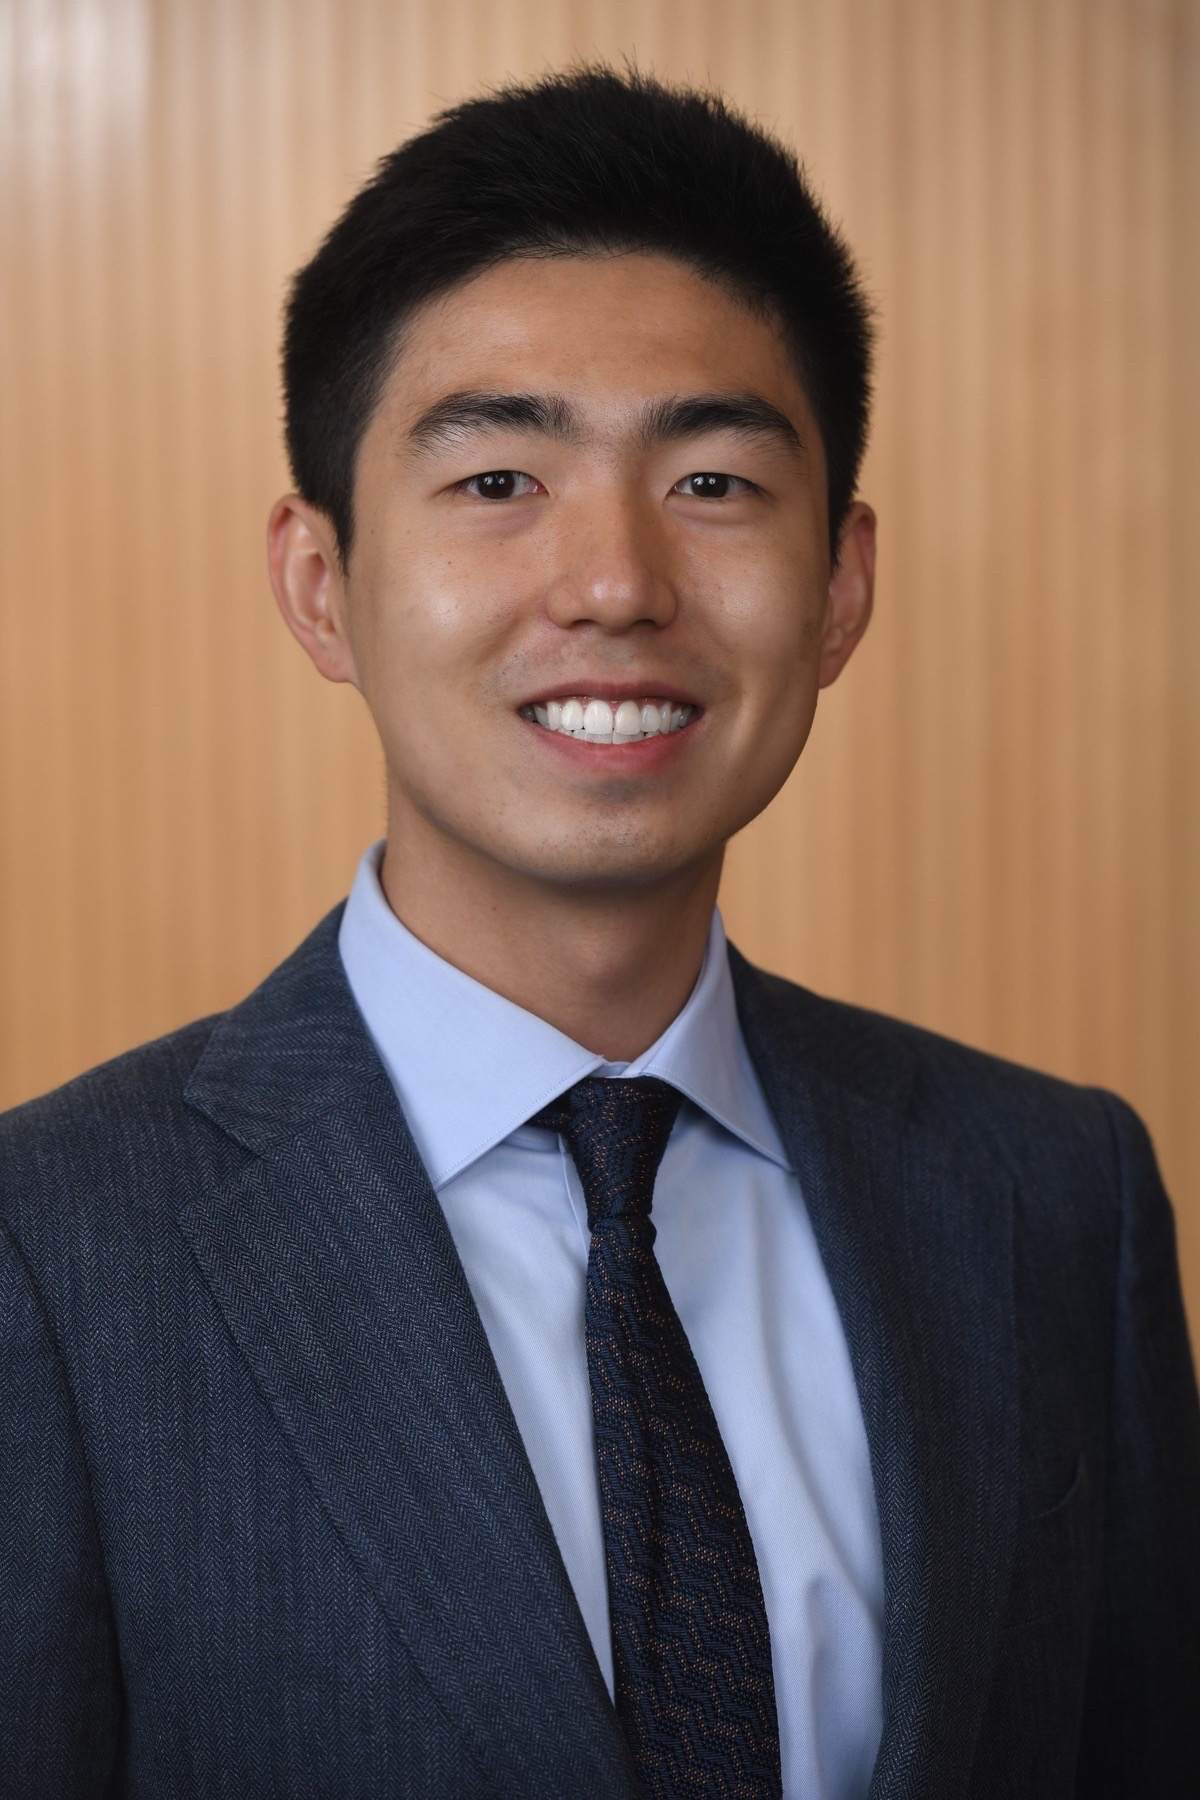
\includegraphics[width=0.3\linewidth]{_pictures/about_us/Jeremy} \caption{me chilling on the beach}\label{fig:unnamed-chunk-1}
\end{figure}

\hypertarget{background-1}{%
\subsection{Background}\label{background-1}}

I was born in Chongqing, a mountainous city in China that's also famous for cyperpunk-like buildings, numbing Szechuan cuisine and spicy hotpot (Yes I love my hometown!). I moved to Beijing with my parents since 10 and live there now. I came to study in the U.S. since 2013, spent 2 years of high school in Vermont, and stayed in New York for 6 years.

I went to New York University for undergrad and graduated with a major in Computer Science and minor in Business Studies. Through various experiences I had developed an interest in data analytics and decided to pivot to data science while developing my business sense.

Now, I am a Master student at Ross School of Business, University of Michigan, studying Business Analytics. I hope to work as a Data Scientist or Data Analyst at an impact-driven tech company after this graduate program and become a Product Manager in 2-3 years.

\hypertarget{favorite-quote}{%
\subsection{Favorite Quote}\label{favorite-quote}}

\begin{quote}
``It's always better to light up a candle than curse the darkness.'' Confucius
\end{quote}

\hypertarget{hobbies}{%
\subsection{Hobbies}\label{hobbies}}

\begin{itemize}
\tightlist
\item
  Weight training
\item
  Basketball
\item
  Running
\item
  Cooking
\item
  Boxing
\item
  Reading
\item
  Movies
\item
  Photography
\item
  Snowboarding
\item
  Wine \& Whiskey tasting
\end{itemize}

\hypertarget{fun-fact}{%
\subsection{Fun Fact}\label{fun-fact}}

\begin{itemize}
\tightlist
\item
  Did sailing in high school
\item
  Was a part of a dragon dance team
\item
  Breakfast is my favorite meal of the day. Just can't live without eggs
\item
  Try to meditate 5 minutes at least every day
\end{itemize}

\hypertarget{business-analyst-101}{%
\chapter{Business Analyst 101}\label{business-analyst-101}}

In this chapter we will cover the following content:
- what is business analytics
- why does it matter for you to know the difference if you are recruiting for a business analyst position

\hypertarget{business-analyst-in-consulting}{%
\chapter{Business Analyst in Consulting}\label{business-analyst-in-consulting}}

In this chapter we will cover the following content:

\begin{itemize}
\tightlist
\item
  what does business analysts do in Consulting industry
\item
  what skillsets are required and preferred
\item
  what is a day-to-day like for a business analyst in Consulting
\item
  how does they work in teams (with other consultants, with clients, etc.)
\end{itemize}

\hypertarget{business-analyst-in-tech}{%
\chapter{Business Analyst in Tech}\label{business-analyst-in-tech}}

In this chapter we will cover the following content:

\begin{itemize}
\tightlist
\item
  what does business analysts do in Tech industry
\item
  what skillsets are required and preferred
\item
  what is a day-to-day like for a business analyst in Tech
\item
  what is the differnece between business analyst, data analyst, data scientist, and machine learning engineer
\item
  how does they work in teams (with engineers and scientists, with stakeholders, with product managers, etc.)
\end{itemize}

\hypertarget{business-analyst-in-finance}{%
\chapter{Business Analyst in Finance}\label{business-analyst-in-finance}}

\hypertarget{content}{%
\section{Content}\label{content}}

In this chapter we will cover the following content:

\begin{itemize}
\tightlist
\item
  what does business analysts do in Finance industry
\item
  what skillsets are required and preferred
\item
  what is a day-to-day like for a business analyst in Finance
\item
  what is the differnece between one's job at an investment bank, private equity, venture capital, commerical bank, etc.
\item
  how does they work in teams
\end{itemize}

  \bibliography{book.bib,packages.bib}

\end{document}
